\documentclass[5p,times,numbers,authoryear]{elsarticle}

\usepackage{ctex}
\usepackage{lineno}%,hyperref}
\usepackage[colorlinks,citecolor=blue]{hyperref}

\usepackage{graphics}
\usepackage{graphicx}
\usepackage{subfigure}
\usepackage{enumitem}
\usepackage{helvet}
\usepackage{courier}
\usepackage{diagbox}
\usepackage{amsmath}
\usepackage{multirow}
\usepackage{booktabs}
\usepackage{makecell}
\usepackage{amssymb}
\usepackage{threeparttable}
\usepackage[justification=centering]{caption}
\usepackage[linesnumbered,ruled,vlined,commentsnumbered]{algorithm2e}
\usepackage{color}
\usepackage{xcolor}
\usepackage{colortbl}
\usepackage{float}
\usepackage{bm}
\usepackage[normalem]{ulem} % use normalem to protect \emph
\newcommand\hl{\bgroup\markoverwith
	{\textcolor{yellow}{\rule[-.5ex]{2pt}{2.5ex}}\ULon}}

\usepackage{hyperref}
\usepackage{breakurl}

\newtheorem{definition}{Definition}
\def\boxend{\hspace*{\fill} $\Box$}
\newcommand{\comment}[1]{}
\renewcommand{\multirowsetup}{\centering}

\journal{Computers in Human Behavior}

\usepackage{appendix}

\begin{document}

\begin{frontmatter}

\title{Stress-Buffering Pattern of Positive Events on Adolescents: \\
An Exploratory Study Based on Social Networks}


\begin{abstract}
Stress is viewed as the leading cause of mental health issues. Positive events, however, could act as a buffer against stress. Since the stress-buffering effects of positive events in previous studies were mainly examined by subjective self-reporting, continuous tracking research at individual behavioral levels still remains to be explored. In this study, we collected microblogs (n=27,346) from a group of high school students (n=500) to examine the relationship between positive events and stress-buffering patterns at both the content and behavioral levels. Through a pilot study of scheduled exam intervals under two situations, namely, 1) existing neighboring positive scheduled events (n=75) and 2) no neighboring positive events, we found that students taking exams with neighboring positive events appeared to exhibit less intense stress and more stable stress fluctuations.
Most students talked less about exams when positive events occurred nearby, at a lower frequency and a lower ratio.
Hypothetical tests for stress-buffering effects of positive events and monotonic changes in the stress intensity under the impact of positive events were further conducted based on automatically extracted positive events (n=1,914) from the microblogs.
The results showed that the stress-buffering effects of positive events were closely correlated with adolescents' stress-change modes, microblog linguistic expressions, and posting behaviors.
The occurrence of positive events was verified to offset the impact of stressor events through talking about positive topics at the same time.
Adolescents tended to post more forwarded microblogs, more positive microblogs and less stressful microblogs when positive events appeared;
however, the total frequency of microblogs did not appear to change significantly under the impact of positive events.
The study also showed that positive events buffered monotonic changes in stress intensity caused by stressor events.
Based on these theoretical findings, the stress-buffering patterns around positive events were further incorporated for stress prediction in adolescents, and the predictive performance was improved.
This study could inform the use of social networks to estimate and track mental health transitions in adolescents under stress. The theoretical and practical implications, limitations of this study and future work are discussed.
\end{abstract}

\begin{keyword}
stress-buffering effect, positive events, microblogs, adolescents
\end{keyword}
\end{frontmatter}

\section{Introduction}
\emph{Motivation}: Life is always full of ups and downs.
Accumulated stress could drain inner resources,
leading to psychological maladjustment, depression and even suicidal behaviors \citep{Nock2008Suicide}.
Compared to adults, 
%Editor: Please ensure that the intended meaning has been maintained in this edit:
{young people exhibit high levels of stress}
due to their immature inner status and lack of experience \citep{older}.
According to the latest report released by the American Psychological Association in 2018,
91\% of young adults had experienced physical or emotional symptoms due to stress in the past month compared to 74\% of adults \citep{APA2018}.
More than 30 million Chinese adolescents suffer from psychological stress,
and nearly 30\% of them are at a risk of depression \citep{ChinaTeen2019}.
Stress-induced mental health problems are becoming an important social issue worldwide.

On the other hand, positive life events, such as satisfying social interactions,
excellent academic performance and pleasant entertainment activities,
could exert protective effects on emotional distress in both direct and indirect ways by \emph{`buffering'} ~\citep{Shahar2002Positive, Cohen2010Positive},
with respect to physiological, psychological, and social coping resources~\citep{Cohen1984Positive,Needles1990Positive}.
Researchers indicated that positive events mitigated the relationship between negative events and maladjustment in samples of adolescents experiencing family transitions \citep{Doyle2003Positive}.
The written expression of positive feelings also prompted increased cognitive reorganization in an undergraduate student group \citep{Coolidge2009A}.
Positive events have also been linked to medical benefits, such as improved mood, serum cortisol levels, and lower levels of inflammation and hypercoagulability \citep{Caputo1998Influence,Jain2010Effects}.
Thus, tracking the state of the stress-buffering effect is important for understanding the mental status of stressed individuals.
%------------

\emph{Existing solutions}:
Previous studies have focused on measuring positive events and stress-buffering states after events through questionnaires.
including the Hassles and Uplifts Scale~\citep{Kanner1981Comparison}, the
Perceived Benefit Scales~\citep{Mcmillen1998The}, the
Interpretation of Positive Events Scale~\citep{Alden2008Social}
and the Adolescent Self-Rating Life Events Checklist~\citep{Jun2008Influence}.
Recently, scholars have demonstrated the feasibility to sense and predict users' stress from social networks~\citep{XueUbicomp13,Xue2014Detecting,Lin2014User,Li2015When,Li2015Predicting,Li2015Using,
Li2017Analyzing,Li2017Exploring}
through content (linguistic text, emoticons, and pictures)
and behavioral (abnormal posting time and comment/response actions) measures.

If we view the aforementioned traditional studies on positive events as static sensing of stress-buffering, this study approaches the problem stress-buffering as a dynamic process
and aims to find a solution at both the microblogging-content and behavioral levels under the hypothesis that the occurrence of positive events can be reflected in adolescents' microblogs.
Subjective self-reported investigations are susceptible to many factors,
such as 
%Editor: Please ensure that the intended meaning has been maintained in this edit here and elsewhere throughout the manuscript':
{social pressure} 
and pressure from measurement scenarios, but
microblogging characteristics at the behavioral level are objective expressions that can assist in identifying content characteristics.

Another difference from the previous studies lies in that, despite the unique advantages of social networks over traditional survey methods in offering self-expressed content and behavioral information, previous microblog-based studies stopped the analysis of stress,
and none went further to capture positive events that may play a key role in adolescents' stress-coping mechanisms.
For example, `hiking tomorrow' might simultaneously occur and be expressed in microblogs with 
%Editor:Please ensure that the intended meaning has been maintained in this edit:
{`failing the exam today'.}
If do not know anything about positive events, is the unilaterally detected stress the real stressful state of the current youth?
Understanding stress-buffering patterns of positive events is helpful in precisely predicting and guiding adolescents who are coping with stress.

\emph{Our work}:
To this end, this paper studies adolescent stress from the dual perspective of stress generation and stress-buffering and views stress as the superposition effect of stressors and positive events.
By investigating the connection between positive events and stress changes
reflected through adolescents' microblogging content and behaviors, we discover stress-buffering patterns around positive events and further predict future stress under such mitigation.
Exploiting the stress-buffering effects of positive events is also advantageous in handling the confusing situation of whether an adolescent who does not express stressful information in microblog is actually under stress.

However, capturing the stress-buffering process of positive events is not a trivial task.
Three fundamental challenges need to be addressed:
1) What are the criteria for depicting 
%Editor: Please ensure that the intended meaning has been maintained in this edit:
{stress-buffering effects?}
2) What is the latent connection between positive events and adolescents' stress-buffering reflections in microblogs?
3) How  can extract positive events and their impact interval be extracted from microblogs?

%1
A pilot study was first conducted on the microblog data (n=27,346) of a group of high school students (n=500) associated with the school's positive scheduled events (n=75) and stressor events (n=122).
Stressful intervals were divided into two comparative categories:
intervals impacted by positive scheduled events (denoted by U-SI, n=259)
and intervals not impacted by positive scheduled events (denoted by SI, n=518).
After observing the posting behaviors and microblog content of the stressed students in both the SI and U-SI groups, several implications were discussed to guide the next step of the study.

%3
Motivated by the implications of the pilot study, we modeled the connection between positive events and adolescents' stress-buffering reflections as the statistical difference in two comparative situations SI and U-SI.
Three groups of measures were adopted to depict adolescent stress buffering at the period level:
stress-change modes, linguistic expressions and posting behaviors.
Positive events buffered monotonic changes in stress intensity.
Monotonic changes in stress intensity buffered by positive events were measured in temporal order.
%4
As an exploration, according to the occurrence of automatically extracted positive events,
we covered the stress-buffering effects into each time unit and integrated such an effect into the stress prediction model.

%2
In this paper, to automatically extract positive events, we built upon and extended previous stress and event detection works. A Chinese linguistic parser model was applied to extract positive events in the linguistic structure
\emph{[type, (act, doer, description)]}.
We followed the categorization of adolescents' positive events in six dimensions (entertainment, school life, romantic, peer relationships, self-cognition, and family life) and extended the 
%Editor: Abbreviations and acronyms are typically defined the first time the term is used within the main text and then used throughout the remainder of the manuscript. Please consider adhering to this convention. The target journal may have a list of abbreviations that are considered common enough that they do not need to be defined:
SC-LIWC 
lexicons into 2,606 phases.
Stressful intervals (SI) and stressful intervals impacted by positive events (U-SI) were identified according to their temporal order.

The rest of the paper is organized as follows.
We review the literature in section \ref{sec:related} and introduce the pilot study in section \ref{sec:obs}.
The procedure for extracting positive events is presented in section \ref{sec:frame1}.
The connection between positive events and adolescents' stress buffering from microblogs are discussed and modeled in section \ref{sec:frame2}.
We present the experimental results in section \ref{subsec:experiment}
and extend the study to integrating stress-buffering patterns into future stress prediction in section \ref{subsec:predict}.
Future work is discussed in section \ref{sec:conclude}.

\section{Literature Review}
\label{sec:related}
\subsection{Stress-buffering Function of Positive Events}
Positive events have been verified as protective factors against daily stress~\citep{Ong2006Psychological,Bono2013Building}, loneliness~\citep{Chang2015Loneliness}, suicide~\citep{Evan2014Social} and depression~\citep{Santos2013The}.
By exploring naturally occurring daily stressors, \citep{Ong2006Psychological} found that over time, the experience of positive emotions assists high-resilient individuals in recovering effectively from daily stress.
Through a three-week longitudinal study, \citep{Bono2013Building} examined the correlation between employee stress and health and positive life events and concluded that naturally occurring positive events are correlated with decreased stress and improved health.
\citep{Chang2015Loneliness} investigated the protective effect of positive events in a sample of 327 adults and found that the positive association between loneliness and psychological maladjustment was weaker for those who experienced a large number of positive life events, as opposed to those who experienced a small number of positive life events.
This finding agrees with the conclusion made by \citep{Evan2014Social} that positive events act as protective factors against suicide individually and synergistically when they co-occurred,
by buffering the link between important individual differences in risk variables and maladjustment.
In the survey conducted by \citep{Santos2013The}, strategies of positive psychology were also identified as potential tools for the prophylaxis and treatment of depression, helping to reduce symptoms and prevent relapses.

The protective effect of positive events was hypothesized to operate in both direct (i.e., the more positive events people experienced, the less stress they perceived)
and indirect ways by \emph{`buffering'} the effect of stressors ~\citep{Cohen2010Positive,Shahar2002Positive},
with respect to physiological, psychological, and social coping resources ~\citep{Cohen1984Positive, Needles1990Positive}.
\citep{Folkman2010Stress} identified three classes of coping mechanisms that were associated with positive emotions during chronic stress: positive reappraisal, problem-focused coping, and the creation of positive events.
Due to their immature inner status and lack of experience,
adolescents exhibit more sensitivity to stressors
(i.e., exams, heavy homework load, isolation by classmates, family transitions),
and live with frequent, long-term stress~\citep{older}.
In this situation, positive events could help reinforce adolescents' sense of well-being~\citep{Coolidge2009A} and
restore the capacity to handle stress~\citep{Doyle2003Positive}
and have also been linked to medical benefits, such as improved mood, serum cortisol levels, and lower levels of inflammation and hypercoagulability \citep{Jain2010Effects,Caputo1998Influence}.
The present study will be based on the consensus conclusions from the above studies.

To assess the stress-buffering effect of positive events,
scholars conducted many studies based on self-support methods.
For example,
\citep{Kanner1981Comparison} developed the Hassles and Uplifts Scale
and concluded that the assessment of daily hassles and uplifts might be a better approach to the prediction of adaptational outcomes than the usual life-events approach.
To measure the negative interpretations of positive social events,
\citep{Alden2008Social} proposed the Interpretation of Positive Events Scale and analyzed 
%Editor: Please review this passage. It seems to be a direct quotation from the cited article. Direct quotations are usually placed in quotation marks and followed by a citation. Another option is to paraphrase the passage in your own words and to include the appropriate citation.
{the relationship between social interaction anxiety and the tendency to interpret positive social events in a threat-maintaining manner.}
\citep{Mcmillen1998The} proposed the Perceived Benefit Scales as new measures of self-reported positive life changes after traumatic stressors, including lifestyle changes, material gain, increases in self-efficacy, family closeness, community closeness, faith in people, compassion, and spirituality.
Specific to college students,
\citep{Jun2008Influence} administered the Adolescent Self-Rating Life Events Checklist  to 282 college students  and found that training in positive coping styles was of great benefit to improve the mental health of students.
The above explorations are based on self-reported investigations; therefore, it is difficult to exclude the interference from external factors (i.e., social pressure and pressure from measurement scenarios).
Moreover, due to the lack of personnel and effective scientific methods,
most scholars have relied on a limited number of measurements;
thus, continuous measurements of the stress-buffering process were difficult to carry out.

\subsection{Measures and Stress Analysis from Social Networks}
As billions of adolescents are recording their lives through social networks (e.g., microblogs, Twitter, and Facebook), researchers have explored applying psychological theories to social network-based data mining techniques to better understand users' psychological statuses from the self-expressed public data source.
Multiple content and user behavioral measures have been 
%Editor: Please consider "suggested", "indicated" or "shown" as a more widely accepted alternative here and throughout the manuscript:
{proven} 
effective in user mental health analysis,
including time series curve analysis of stress~\citep{Li2015When,Li2015Using}, topic words~\citep{XueUbicomp13}, abnormal posting time~\citep{Xue2014Detecting},
online shopping behaviors~\citep{DBLP:conf/apweb/Zhao0XLF16},
human mobility features~\citep{DBLP:conf/dasfaa/JinXLF16}, comment/response actions~\citep{Liang2015Teenagers}
and high-dimensional multimedia features~\citep{Lin2014User}.
For example, \citep{XueUbicomp13, Xue2014Detecting} proposed detecting adolescent stress from a single post utilizing machine learning methods by extracting topic words indicating stress, abnormal posting time, and interactions with friends.
\citep{Lin2014User} constructed a deep neural network to combine the high-dimensional   semantic information into stress detection.
Based on the stress detection results,
\citep{Li2015Predicting}\cite{Li2015Using}\cite{Li2015When} adopted a series of multivariate time series prediction techniques (i.e., candlestick charts, fuzzy candlestick lines, and seasonal autoregressive integrated moving average models) to predict future stress trends.
Taking  linguistic information into consideration,
\citep{Li2017Exploring} employed a nonlinear autoregressive with external input neural network to predict a teenager's future stress level by referring to the impact of co-experienced stressor events of similar companions.
\citep{Li2017Analyzing} proposed detecting stressor events from microblog content
and analyzing stressful intervals based on the posting rate.
All of the above studies focused on the discussion of stress detection in social networks.
This paper starts from a completely new perspective and focuses on the stress-buffering effect of positive events in adolescents' stress coping processes.
Thus, we extend the study from how to find stress to the next, more meaningful, stage: how to cope with stress.

\subsection{Correlation Analysis Models for Multivariate Time Series}
Basic correlation analysis models on time series focusing on univariate data have been well studied.
As the most widely adopted model, the Pearson correlation coefficient \cite{Cohen1988Statistical} measures the linear correlation between two variables $X$ and $Y$.
One inevitable defect of the Pearson correlation coefficient is its sensitivity to outliers.
To overcome such drawbacks, Spearman's rank correlation coefficient \cite{C1987The} and the Kendall rank correlation coefficient \cite{Mcleod2011Kendall} were proposed based on the Pearson correlation coefficient.
While the Pearson correlation coefficient estimates linear relationships,
Spearman's correlation coefficient estimates monotonic relationships (regardless of linearity),
and are calculated as the Pearson correlation coefficient between the rank values of two variables.
The Kendall rank correlation coefficient mainly assesses the similarity of the orderings of the data when ranked by each of the quantities.
The above correlation metrics are primarily used to estimate the relationship between single-dimensional variables, and cannot be adopted directly in social network-based scenarios.

For multivariate time series analysis, two-sample models are widely adopted.
Such models are built to check whether two samples come from the same underlying distribution,
which is assumed to be unknown.
Correspondingly, various kernel- \citep{Sch2006A} and distance-based models \citep{Schilling1986Multivariate} have been proposed.
\citep{Sch2006A} proposed to transform the distance between two variables and nearest neighbors into a reproducing kernel Hilbert space and to solve the problem using the maximum mean discrepancy.
\citep{Schilling1986Multivariate} adopted an $r$-nearest-neighbor-based model to partition two sets of event-driven time series data.
The global proportion of 
%Editor: Please consider replacing the following text with "right-censored neighbors":
{right divided neighbors} 
was calculated to estimate whether there existed a statistically significant difference between the two sets.
This paper adopted an $r$-nearest-neighbor-based two-sample model in our problem to measure the distance and correlation between two multidimensional variables depicting
the stress-buffering patterns of positive events.

\section{Data Observation: A Pilot Study on the Stress-buffering Effect of School-Scheduled Positive Events}
\label{sec:obs}
\paragraph{Microblogs} Microblogs of students from Taicang High School were collected from January 1, 2014, to September 1, 2017.
We filtered out 121 active students out of over 500 students according to their posting frequency 
and collected their microblogs throughout their whole high school career.
In total, 27,346 microblogs were collected in this study, where each student post an average of 226 microblogs, and maximum of 1,421 microblogs and a minimum of 102 microblogs.
To protect the privacy, all the usernames were anonymized during the experiment.

\paragraph{Scheduled events} The list of weekly scheduled school events,
with a detailed description of the event (grade and exact start and end time),
were collected from the school's official website\footnote{http://stg.tcedu.com.cn/col/col82722/index.html} from February 1, 2014, to August 1, 2017.
There were 126 stressor events and 75 positive events in total.
Examples of positive scheduled  and stressor events in high school life are listed in Table~\ref{tab:example}.
There were 2-3 stressor events and 1-2 positive events scheduled per month in the current study.
Figure~\ref{fig:example} shows three examples of a student's stress fluctuations around three midterm exams, where a positive event \emph{campus art festival} was scheduled ahead of the first exam (\emph{example a}),
A positive event \emph{holiday} occurred after the second exam (\emph{example b}),
and no positive scheduled event was found near the third exam (\emph{example c}).


\begin{table}[H]
\caption{\small{Examples of school-scheduled positive and stressor events.}}
\label{tab:example}
\resizebox{.45\textwidth}{9mm}{
\small{
\begin{tabular}{cccc}
\toprule
Type & Date	& Content	& Grade	\\
\midrule
stressor event & 2017/4/16 & first day of the mid-term exam & grades 1 and 2\\
positive event & 2016/11/5 & campus art festival & grades 1, 2, and 3\\
\bottomrule
\end{tabular}
}
}
\end{table}

\begin{table}[h]
\centering
\caption{\small{Examples of academic-related keywords.}}
\label{tab:studyWords}
\small{
\begin{tabular}{c}
\toprule
exam, fail, review, score, test paper, rank, pass, math, chemistry\\
homework, regress, fall behind, tension, stressed out, physics,\\
nervous, mistake, question, puzzle, difficult, lesson, careless\\
\bottomrule
\end{tabular}
}
\end{table}


\begin{figure}[H]
\centering
\includegraphics[width=\linewidth]{figs/exampleWave.eps}
\caption{\small{Examples of school-scheduled positive events, stressor events, and a student's stress fluctuations}}
\label{fig:example}
\end{figure}

To further observe the effect of positive events on stressed students,
we collected all the stressful intervals surrounding the scheduled exams for the 121 students during their high school career, applying the interval detection method from ~\citep{Li2017Analyzing}.
For each student, we divided all the stressful intervals into two sets:
1) In the original sets, stress was caused by a stressor event, lasting for a period,
and no other intervention (namely, a positive event) occurred.
We called the set of such stressful intervals \textbf{SI};
2) In the other comparative sets, the stressful interval was impacted by a positive event.
We called the set of such stressful intervals \textbf{U-SI}.
Thus, the difference under the two situations (sets) could be seen as the stress-buffering effect
induced by the positive event.
We identified 518 exam-related stressful intervals (SIs)
and 259 stressful intervals impacted by four typical positive scheduled events (U-SIs)
%Editor: Please note that this text and other quotes have been lightly edited. If the quoted material was originally provided in English, please review the quotation for accuracy and reject the changes as necessary:
(`practical activity', `New Year party', `holiday', `sporting event') from the students' microblogs.
Six measures for the above two conditions were considered: 
the \emph{accumulated value of stress}, the \emph{average value of stress} (per day),  the \emph{maximal value of stress} (per day), the \emph{RMS value of stress},
the \emph{frequency of academic topic words}, and the \emph{ratio of academic stress among all types of stress}.
Since our target was to track the impact of positive events for students under stress,
based on previous research~\cite{XueUbicomp13}, we detected the stress level (ranging from 0 to 5) for each post.
For each student, the stress value per day was aggregated by calculating the average amount of stress from all the posts.
Examples of academic-related keywords are listed in Table \ref{tab:studyWords}.
The average value of each measure over all eligible slides was calculated.


\begin{figure}[h]
\centering
\includegraphics[width=\linewidth]{figs/barUSI.eps}
\caption{\small{Comparing stress (average value for all students) during the exam intervals in two situations:
1) intervals affected by positive neighboring events (U-SI) and 2) no positive events occurred nearby (SI).}}
\label{fig:frequencyBar}
\end{figure}

\begin{figure}[h]
\centering
\includegraphics[width=\linewidth]{figs/activity.eps}
\caption{\small{Comparing students' stress fluctuations during exam intervals in the U-SI and SI sets. }}
\label{fig:frequency}
\end{figure}

\paragraph{Results}
As shown in figure~\ref{fig:frequencyBar}, comparing each measure of scheduled exam intervals under the two situations (
1) existing positive neighboring events (U-SI) and 2) no neighboring positive scheduled events (SI)), we found that students with exams and positive neighboring events appeared to exhibit less stress intensity (78.13\% reduction in average stress, 95.58\% reduction in cumulative stress, and 57.20\% reduction in maximal stress) and more stable stress fluctuations (47.93\% reduction in the RMS values of stress).
Furthermore, the frequency of academic topic words (see Table \ref{tab:studyWords} for examples) and the ratio of academic stress in each interval were calculated.
Most students talked less about exams when positive events occurred nearby 
with lower frequency (84.65\% reduction) and lower ratio (89.53\% reduction).
The statistical results show clues about the impact of positive scheduled events,
which is consistent with psychological theory ~\citep{Cohen1984Positive, Cohen2010Positive, Needles1990Positive}, indicating the reliability and feasibility of the microblog dataset.
However, this observation is based on specific scheduled events,
and cannot satisfy the need for automatic, timely, and continuous perception of the stress-buffering process.
Therefore, we propose a framework to automatically detect positive events and their impact interval.
Based on this framework, the relationship between the impact of automatically extracted positive events and adolescents' microblogging characteristics will be discussed.


\section{Framework}
\label{sec:frame}
We first introduce the procedure to extract positive events and their intervals from microblogs.
Based on this procedure, we present a statistical model to depict the relationship between positive events and adolescents' stress-buffering patterns through three groups of content and behavioral measures.
%Finally, a none-liner time series model was proposed to combine stress-buffering patterns into future stress prediction.
\subsection{Discovery of Positive Events from Microblogs}
\label{sec:frame1}
Let $u$ = $[type,\{doer, act,$ $description\}]$ be a positive event,
where the element \emph{doer} is the subject who performs the \emph{act},
and \emph{description} is the key words related to $u$.
According to psychological scales ~\citep{Jun2008Influence,hassles},
positive events for adolescents mainly focus on six dimensions:  $\mathbb{U} =\{$ `entertainment', `school life', `romantic relationships', `peer relationships', `self-cognition', `family life'$\}$. We constructed our lexicon for six-dimensional positive events from two sources.
The basic positive words are selected from the psychological lexicon C-LIWC (expectation, joy, love, and surprise)~\citep{Tausczik2010The}.
Then, we built six topic lexicons by expanding basic positive words from the adolescents' microblogs, containing 452 phrases in `entertainment',
273 phrases in `school life',
138 phrases in `romantic relationships',
91 phrases in `peer relationship',
299 phrases in `self-recognition' and 184 phrases in `family life', for a total of 2,606 phrases. 
Examples are shown in Table \ref{tab:topicWords}.
Additionally, we labeled \emph{doer} words (i.e., \emph{teacher}, \emph{mother}, \emph{I} and \emph{we}) in positive lexicons.

\begin{table*}
\centering
\caption{\small{Examples and statistics for topic phrases in the six-dimensional lexicons of positive events.}}
\label{tab:topicWords}
\small{
\begin{tabular}{lll}
\toprule
Dimension & Example words & Total \\ \midrule
entertainment  & hike, travel, celebrate, dance, swimming, ticket, shopping, air ticket, theater, party, karaoke,& 452\\
                      & self-driving tour, game, idol, concert, movie, show, opera, baseball, running, fitness, exercise & \\
school life    & reward, come on, progress, scholarship, admission, winner, diligent, first place, superior & 273\\
				      & hardworking, full marks,  praise, goal, courage, progress, advance, honor, collective honor& \\
romantic relationships      &  beloved, favor, guard, anniversary,  concern, tender, deep feeling, care, true love, promise, & 138\\
				      & cherish, kiss, embrace, dating, reluctant, honey, sweetheart, swear, love, everlasting, goddess &\\
peer relationships  & listener, company, pour out, make friends with, friendship, intimate, partner, teammate, brotherhood& 91\\
self-cognition & realize, achieve, applause, fight, exceed, faith, confidence, belief, positive, active, purposeful & 299\\
family life    & harmony, filial, reunite, expecting, responsible, longevity, affable, amiability, family, duty & 184\\
\bottomrule
\end{tabular}}
\end{table*}

\begin{table}[h]
\begin{center}
\caption{\small{Examples of automatically extracted positive events from the adolescents' microblogs.}}
\small{
\begin{tabular}{|l|} \hline
I am really looking forward to the spring outing on Sunday. \\
(doer: \emph{I}, act: \emph{looking forward}, description: \emph{spring outing})\\\hline
My holiday is finally coming [smile]. \\
(doer: \emph{My holiday}, act: \emph{coming}, description: \emph{[smile]})\\\hline
First place on my lovely math exam!!! In memory of it.\\
(description: \emph{first place, math, exam, memory})\\\hline
You are always here for me like sunshine. \\
(doer: \emph{You}, description: \emph{sunshine})\\\hline
Thanks to all my dear friends for hosting the party.
Happiest birthday!!!\\
(doer: \emph{friends}, act: \emph{thanks}, description: \emph{party, birthday})\\\hline
I know my mom is the one who will support me forever, no matter \\
when and where. (doer: \emph{mom}, act: \emph{support})\\ \hline
Expecting tomorrow's Adult Ceremony [smile] [smile]~~\\
(act: \emph{expecting}, description: \emph{Adult Ceremony})\\\hline
\end{tabular}}
\label{tab:uplifts}
\end{center}
\end{table}

\subsubsection{Linguistic Parser Model}
Positive events were identified through a Chinese natural language processing platform \citep{Che2010}.
For each post, after word segmentation, we parsed each sentence to find its linguistic structure
and then matched the main linguistic components with positive topic lexicons in each dimension.
A linguistic parser model was applied to identify the central verb of the current sentence, namely, the \emph{act}.
It constructed the relationship between the central verb and corresponding \emph{doer} and \emph{description} elements.
By searching these elements in positive topic lexicons, the existence of positive events was identified.
Due to the sparsity of posts, the element \emph{act} might be empty.
\emph{Descriptions} were collected by searching all nouns, adjectives and adverbs.
Examples of positive events extracted from the adolescents' microblogs are listed in table \ref{tab:uplifts}.
For example, the post `Thanks all my dear friends for hosting the party. Happiest birthday!!!'
was processed as \emph{doer=`friends', act = `expecting', description = `party'},
and \emph{type = `entertainment'}.

\subsubsection{Impact Intervals of Positive Events}
\label{subsec:interval}
We followed and extended the method in ~\citep{Li2017Analyzing} to identify the impact interval of each positive event to further study its stress-buffering pattern.
The target interval was identified in three steps.

Step 1:
Positive events, stressor events and filtered-out candidate intervals were extracted.
For each candidate interval, we set its length to more than 3 days and a maximum gap of 1 day between two neighboring stressful days.
Since the stress series detected from the microblogs were discrete points, the locally weighted regression ~\citep{Cleveland1988Locally} method was adopted to highlight the characteristics of the stress curve.

Step 2: 
Intervals were judged as stressful or not through hypothesis testing.
A Poisson-based probability model was adopted to measure how confident we are that the current interval was a stressful interval.
Here, the stressful posting rates under stressful $\lambda_1$ and normal conditions $\lambda_0$ were modeled as two independent Poisson processes:
\begin{equation}
Pr[N=n|\lambda_i]=\frac{e^{-\lambda_i T}{(\lambda_i T)}^n}{n!}
\end{equation}
where $i\in\{0,1\}$ and $n=0,1,\cdots,\infty$.
We expected that $\lambda_1 > \lambda_0$ and measured the probability as $P(\lambda_1>\lambda_0|N_1, T_1, N_0, T_0)$,
where $N_1$ and $N_0$ are the numbers of stressful posts and $T_1$ and $T_0$ are the time durations corresponding to $\lambda_1$ and $\lambda_0$, respectively.
Without loss of generality, we assume a Jeffreys noninformative prior on $\lambda_1$ and $\lambda_0$ and infer the posterior distribution $P(\lambda_1|N_1)$ and $P(\lambda_0|N_0)$ according to Bayes' Rule.
Thus, for the current interval $I_1$ and historical normal interval $I_0$, the quantified probability $\beta = P(\lambda_1>\lambda_0|I_1,I_0)$ $\in (0,1)$ indicates confidence in 
whether $I_1$ was a stressful interval.

Step 3: The stressful intervals were divided into an SI set and a U-SI set.
For a detected stressful interval $I = <t_1,\cdots,t_n>$, we considered the temporal order between $I$ and any detected positive event $u$ occurring at time point $t_u$ in three cases:
\begin{itemize}
\item[1)] If the positive event $u$ occurred during the stressful interval, i.e., $t_u \in [t_1,t_n]$, the positive interval $I$ was judged as $I \in U-SI$.
\vspace{-0.3cm}
\item[2)] If the positive event occurred near a stressful interval, the probability that it had an impact on the current stressful interval was considered.
Here, the gap between $t_u$ and $I$ is limited to $\xi$, i.e.,
if $t_u \in [t_{1}-\xi, t_1)\cup(t_{n},t_{n}+\xi]$, then $I \in U-SI$.
If a stressful interval satisfies none of the above conditions, we classify it into the SI set.
\vspace{-0.3cm}
\item[3)] Other stressful intervals were classified into the U-SI set.
\end{itemize}

\subsection{Hypothesis Test for the Relationship Between Positive Events and Adolescents' Stress-buffering Patterns}
\label{sec:frame2}
We formulated the relationship between positive events and adolescents' stress-buffering patterns as a comparison problem between two sets of stressful intervals: the SI set and the U-SI set.
Each interval was modeled as a multidimensional vector depicting the microblogging characteristics of the current adolescent.
Specifically, a multivariate two-sample hypothesis test 
\cite{Li2017Correlating,Johnson2012Applied} was adopted to model such a relationship.
The basic idea was to determine whether the multidimensional points (i.e., the stressful intervals)
in set SI and set U-SI follow different statistical distributions.
Assuming the data points in SI and U-SI were randomly sampled from distribution $F$ and $G$, respectively, then the hypothesis can be denoted as follows:
\begin{equation}
H_0: F = G \quad versus \quad H_1: F \neq G.
\end{equation}
Under such a hypothesis,
$H_0$ indicates that points in SI and U-SI follow a similar distribution,
while $H_1$ means points in SI and U-SI follow statistically different distributions,
namely, positive events had obvious stress-buffering effects.

\subsubsection{Statistical Model of the Stress-buffering Effect}
\begin{figure*}
\centering
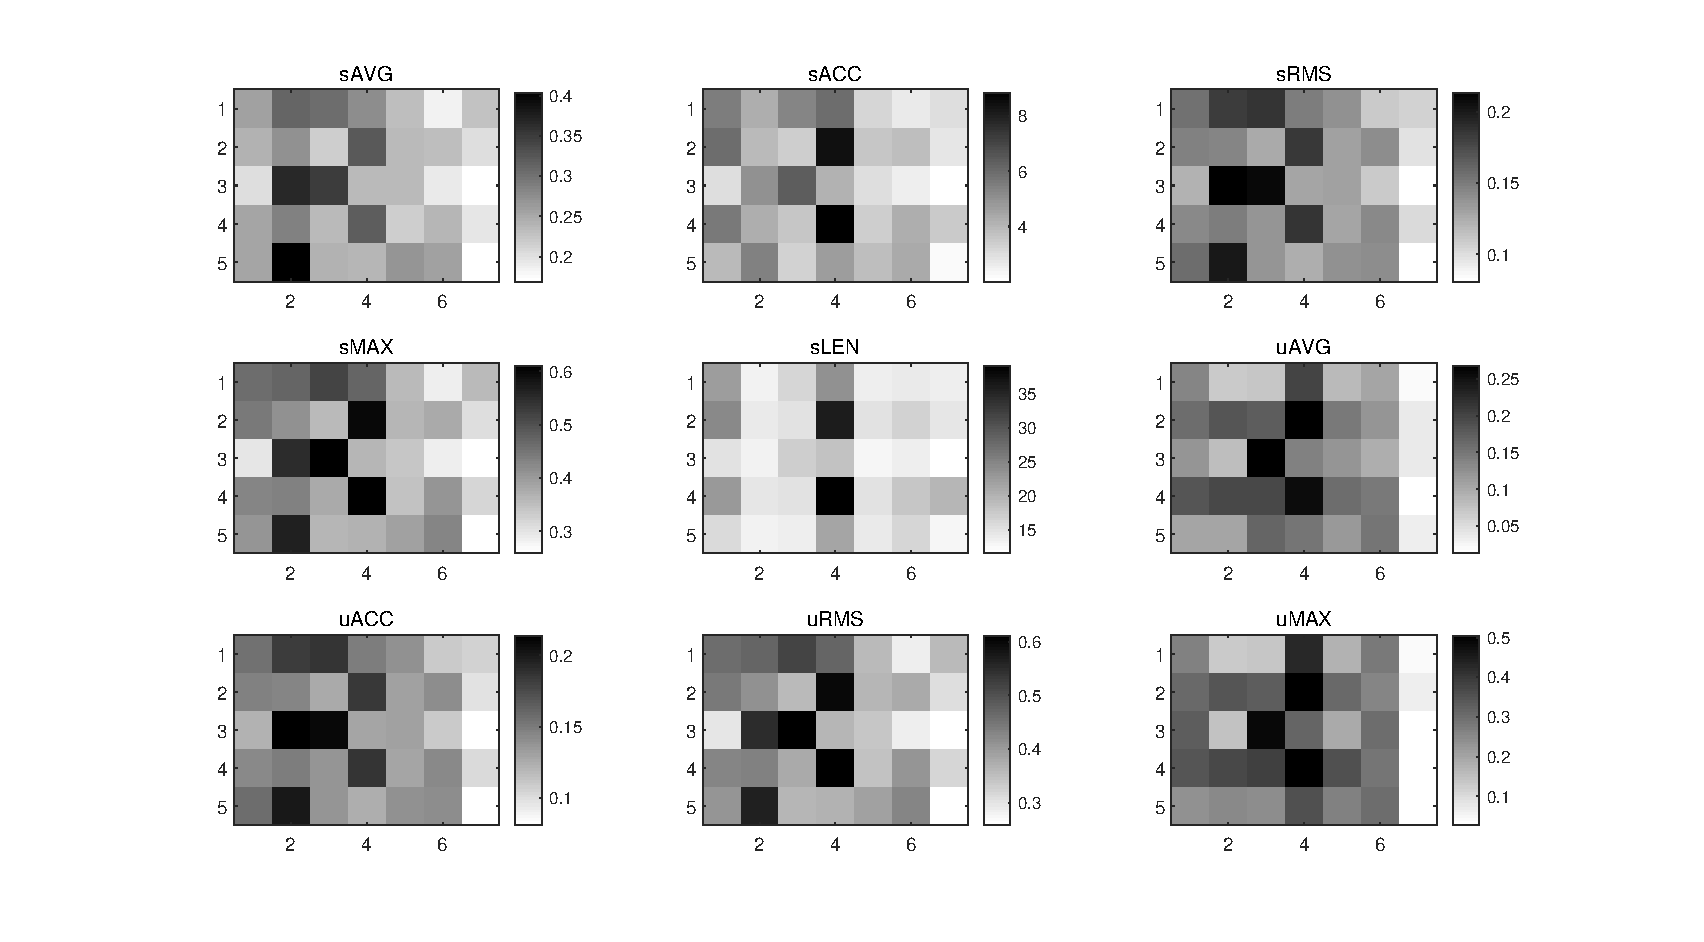
\includegraphics[width=\linewidth]{figs/gray/stress.eps}
\caption{\small{Comparing stress-change modes during stressful intervals in two situations:
1) intervals affected by positive neighboring events (U-SI) and 2) no positive events occurred nearby (SI).
$P_{1-6}$=\{school life, romantic relationships, peer relationships, self-cognition, family life, entertainment\},
$E_{1-5}$=\{school life, romantic relationships, peer relationships, self-cognition, family life\}.}}
\label{fig:stress}
\end{figure*}
We used a K-nearest-neighbor-based method (\cite{Schilling1986Multivariate}) to judge the existence of a significant difference between set SI and set U-SI.
For simplification, we used the symbol $A_1$ to represent set SI and $A_2$ to represent set U-SI.
For each point $\ell_{x}$ in the two sets, we expected its top-k similar points to belong the same set of $\ell_x$.
The Euclidean distance was adopted to calculate the distance of structured points here.
For each point $\ell x \in A=A_1\bigcup A_2$, let $\textbf{D}^y$ be the feature vector of $\ell_x$ and $NN_r(\ell_x,A)$ be the function to find the $r-$th nearest neighbor of $\ell_x$.
The $r$-th nearest neighbor of $\ell_x$ was denoted by:
\begin{equation}
\begin{aligned}
& NN_r(\ell_x,A) = \{y | min\{||\textbf{D}^x-\textbf{D}^y ||_2\}, y\in(A/\ell_x)\} &
\end{aligned}
\end{equation}
Let $I_r(\ell_x,A1,A2)$ be the function denoting whether the $r$-th nearest neighbor was in the same set as $\ell_x$:
\begin{equation}
I_r(\ell_x,A_1,A_2) =
\left\{ \begin{array}{ll}
1, \quad if \ell_x \in A_i  \&\& NN_r(\ell_x,A)\in A_i,\\
0, \quad otherwise
\end{array}
\right.
\end{equation}
Let $T_{r,n}$ denote the proportion that pairs containing two points from the same set among all pairs formed by $\ell_x \in A$ and its $k$ nearest neighbors:
\begin{equation}
T_{k,n}= \frac{1}{n\times k}\sum_{i=1}^{n}\sum_{j=1}^{k}I_j(x,A_1,A_2)
\end{equation}
The value of $T_{k,n}$ showed how differently the points in the two testing sets (SI and U-SI) performed.
If the value of $T_{r,n}$ was close to $1$, then the two underlying distributions $F$ and $G$ for $SI$ and U-SI were significantly different, indicating current positive events had an obvious stress-buffering impact on the adolescents' stress series.
Let $\lambda_1=|A_1|$ and $\lambda_2=|A_2|$, the statistical value $Z$ is denoted by:
\begin{align}
&Z=(nr)^{1/2}(T_{r,n}-\mu_{r})/\sigma_{r}\\
&\mu_r=(\lambda_1)^2+(\lambda_2)^2\\
&{\sigma_r}^2=\lambda_1\lambda_2+4{\lambda_1}^2{\lambda_2}^2
\end{align}
where $\mu_r$ is the expectation and ${\sigma_r}^2$ is the variance of $Z$.
Based on hypothesis testing theory (\cite{Johnson2012Applied}), when the size of the testing set is large enough, $Z$ obeys a standard Gaussian distribution.
Thus, we judged whether the positive events had a significant stress-buffering impact as follows:
if $f(SI,USI)=(nr)^{1/2}(T_{r,n}-\mu_{r})/{\mu_r}^2>\alpha$ ($\alpha = 1.96$ for $P=0.025$),
then the hypothesis $H_1$ was true.

In section \ref{subsubM}, three groups of microblogging measures
were introduced to depict the multidimensional characteristics of each stressful interval $\ell_x$ $\in A$, indicated as an linguistic expression matrix \bm{${D_l^x}$}, a posting-behavior matrix \bm{${D_p^x}$} and a stress-change-mode matrix \bm{${D_s^x}$}.
Correspondingly, three subfunctions of $NN_r(.)$ were defined: $PNN_r(.)$, $SNN_r(.)$ and $LNN_r(.)$.
\begin{equation}
\begin{aligned}
& PNN_r(\ell_x,A)
= \{y | min\{||\textbf{D}_p^x-\textbf{D}_p^y ||_2\}, y\in(A/\ell_x)\} &\\
& SNN_r(\ell_x,A)
= \{z | min\{||\textbf{D}_s^x-\textbf{D}_s^z ||_2\}, z\in(A/\ell_x)\} \\
& LNN_r(\ell_x,A)
= \{w | min\{||\textbf{D}_l^x-\textbf{D}_l^w ||_2\}, w\in(A/\ell_x)\} &
 \end{aligned}
 \end{equation}
The $r$-th nearest neighbor was recalculated as:
\begin{align}
&NN_r(\ell_x,A) = \{v | min\{a \times ||\textbf{D}_p^x-\textbf{D}_p^v||_2+\\
&b \times ||\textbf{D}_s^x-\textbf{D}_s^v||_2+
c \times ||\textbf{D}_l^x-\textbf{D}_l^v||_2\}, v\in(A/\ell_x) \}
\end{align}
In this study, we set $a = b = c = 1/3$.


\subsubsection{Measures}
\label{subsubM}
\paragraph{\textbf{Stress-change modes}}
Inspired by the pilot study, four measures were adopted to quantify the intensity of stress changes during a stressful interval: the average value of stress, the accumulated value of stress, the RMS value of stress, and the maximal value of stress.
For an interval $I=<t_1,t_2,\cdots,t_n>$ with length $|I|=n$ (day), the stress series was denoted by $S=<s_1,s_2,\cdots,s_n>$, where $s_i \in S$ is the average stress value of microblogs posted on day $i$.
The four measures are denoted as follows:
\begin{equation}
\begin{aligned}
&V_{accumulate}(I)= \sum_{i=1}^{n}(s_i)&\\
&V_{average}(I)= \frac{1}{n}V_{accumulated}(I)&\\
&V_{RMS}(I) = \sqrt[2]{ \frac{1}{n}\sum_{i=1}^{n}{(s_i)^2}}&\\
&V_{maximal}(I) = max(I) = \{s_i |\forall s_j \in I \& j \neq i, s_i \geq s_j\}&\\
 \end{aligned}
 \end{equation}
Similarly, we applied the four measures to positive emotional fluctuations in an interval,
which might reflect the complementary changes to stress.
To show the occurrence of the abovementioned measures, we present a 7$\times$5 grayscale map for each measure in Figure \ref{fig:stress}.
The x-axis (ranging from P1 to P6) represents each dimension of positive events
($P$=\{school life, romantic relationships, peer relationships, self-cognition, family life, entertainment\}), and the last column represents no positive events occurring in the observed interval.
The y-axis (ranging from S1 to S5) represents each dimension of stressor events
($E$=\{school life, romantic relationships, peer relationships, self-cognition, family life\}).
The color of each point in the grayscale map depends on the average value of the current measure over the corresponding set of intervals.
For a set of intervals $\textbf{I}_{<e,p>} = <I_1,I_2,\cdots,I_m>$, where the stress was caused by stressor events $e \in E$ and impacted by positive events $p \in P$, the measures are presented as follows:
\begin{equation}
\begin{aligned}
& V_{accumulated}(\textbf{I}_{<e,p>})=\sum_{i=1}^m{V_{accumulated}I_i}&\\
& V_{average}(\textbf{I}_{<e,p>})=\frac{1}{m}\sum_{i=1}^m\I_i&\\
& V_{RMS}(\textbf{I}_{<e,p>})=\sqrt{\frac{1}{m}\sum_{i=1}^mI_i^2}&\\
& V_{maximal}(\textbf{I}_{<e,p>}) = \{max(V_{maximal}(I_i))|i\in[1,m]\} &
 \end{aligned}
 \end{equation}
For example, in Figure \ref{fig:stress} (a), point (P4,S1) is the average stress value in all $\textbf{I}_{<1,4>}$ intervals,
where stress was caused mainly by school life (S1) and impacted by positive events related to self-cognition (P4).
Figure \ref{fig:stress} exhibited four stress-change modes (subgraphs (a) to (d))
and four corresponding positive emotion change modes (subgraphs (e) to (h)) in both the SI and U-SI sets.
The statistical results showed that the occurrence of positive events significantly
reduced the 
%Editor: Please ensure that the intended meaning has been maintained in this edit:
{average stress (subgraph (a))}, 
accumulated stress (subgraph (b)) and maximal stress (subgraph (d)),
and slowed down the fluctuations (subgraph (c)) during stressful intervals.
On the other hand,
the occurrence of positive events caused an obvious increase in all the positive-change modes (subgraphs (e) to (h)),
especially in stressful intervals caused by romantic and self-cognition events.
The above statistics on stress and positive-intensity change modes
initially reflected stress-buffering effects of different types of positive events on each dimension of stressor events.

\begin{figure}[h]
\centering
\includegraphics[width=\linewidth]{figs/gray/emotion.eps}
\caption{\small{Comparing stressful emotions and positive emotions during stressful intervals in the SI and U-SI sets.
$P_{1-6}$=\{school life, romantic relationships, peer relationships, self-cognition, family life, entertainment\},
$E_{1-5}$=\{school life, romantic relationships, peer relationships, self-cognition, family life\}.
}}
\label{fig:topicAll}
\end{figure}

\begin{figure}[h]
\centering
\includegraphics[width=\linewidth]{figs/gray/topicOffset.eps}
\caption{\small{Offset frequency of topic words during stressful intervals in the SI and U-SI sets.
$P_{1-6}$=\{school life, romantic relationships, peer relationships, self-cognition, family life, entertainment\},
$E_{1-5}$=\{school life, romantic relationships, peer relationships, self-cognition, family life\}.}}
\label{fig:stopic}
\end{figure}

\paragraph{\textbf{Linguistic expressions}}
For each microblog, we identified its linguistic expressions applying the segmentation model and parser model from section \ref{sec:frame1}.
The first measure was the frequency of stressful emotional words based on four categories (anger, anxiety, hate, sad) from LIWC lexicons, representing general stress during an interval ~\citep{Tausczik2010The}.
The second measure was the frequency of positive emotional words,
which were identified based on the surprise, joy, expectation and love categories of the LIWC lexicons.
The third measure was the frequency of topic words in the five dimensions of stressor events,
representing the degree of attention for each dimension of stressor events.
Figure \ref{fig:topicAll} (a) and (b) shows the frequency of stressful emotional words and positive emotional words, respectively.
Generally, positive events showed stress-buffering effects in these two measures,
since the last column in subgraphs (a) and (b) was different compared to columns P1 to P6.
Specifically, positive events from romantic, peer relationship and family life showed obvious
reductions in stressful emotional words caused by peer relationship and family life stressor events (subgraph \ref{fig:topicAll} (a)).
Figure \ref{fig:stopic} shows the distribution of stressful topic words when different positive events occurred.
Here, we shows the statistical results during stressful intervals caused by school-life and self-cognition stressor events.
The frequency of stressful academic topic words (subgraphs (a1) and (b1))
and positive academic topic words (subgraphs (a2) and (b2)) showed no clear regularity.
Furthermore, we explored the offset for each dimension of stressful and positive topic words,
as shown in subgraphs (a3) and (b3).
The offset results showed obvious stress-buffering results 
because stressful topic words showed a decrease in columns P1 to P5 in subgraph (a3),
and positive topic words exhibited increases in columns P1 to P5 in subgraph (b3).
These findings reveal that the occurrence of positive events offset the impact of stressor events by simultaneously discussing positive topics.

\begin{figure}[h]
\centering
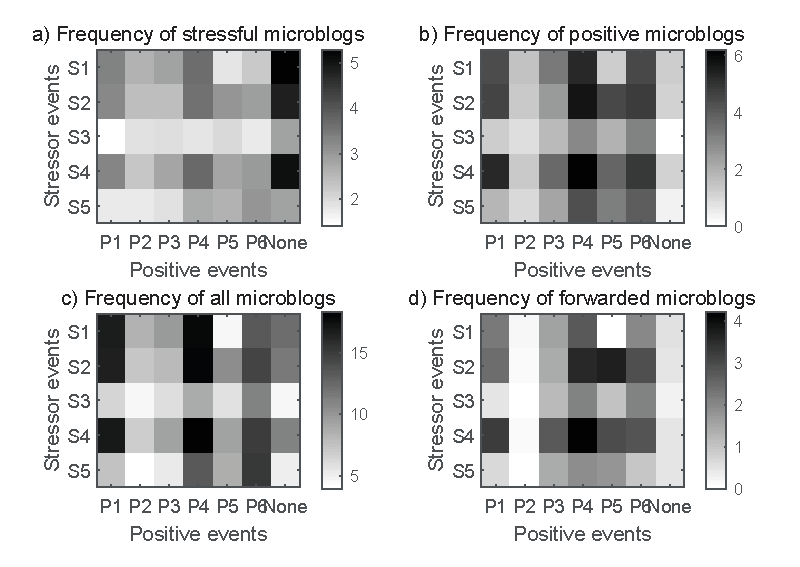
\includegraphics[width=\linewidth]{figs/gray/post.eps}
\caption{\small{Comparing posting behaviors during stressful intervals in the SI and U-SI sets.
$P_{1-6}$=\{school life, romantic relationships, peer relationships, self-cognition, family life, entertainment\},
$E_{1-5}$=\{school life, romantic relationships, peer relationships, self-cognition, family life\}.}}
\label{fig:post}
\end{figure}

\paragraph{\textbf{Posting behaviors}}
Stress can lead to abnormal posting behaviors,
reflecting users' changes in social engagement activities ~\citep{Liang2015Teenagers}.
We considered four measures of posting behaviors here.
The first measure was the frequency of stressful microblogs,
highlighting stressful microblogs among all microblogs.
Research in \cite{Li2017Analyzing} indicated that overwhelmed adolescents
tended to post more microblogs expressing their stress for release and to seek comfort from friends.
The second measure was the frequency of positive microblogs,
indicating the number of positive microblogs per day.
The third measure was the total number of all microblogs per day.
The fourth measure was the frequency of forwarded microblogs,
showing the number of retweets and shared microblogs.
Figure \ref{fig:post} summarizes the distribution of the above four measures in the U-SI and SI sets.
The results in subgraphs (a) and (b) show a decrease in stressful microblogs and an
increase in positive microblogs when positive events occurred.
Subgraph (d) indicates that adolescents tended to forward more microblogs when positive events occurred, 
while subgraph (c) showed that the frequency of all microblogs did not appear to change significantly under the impact of positive events.

\begin{table*}
\begin{center}
\caption{\small{Monotonic stress-intensity changes in the U-SI and SI intervals compared with adjacent intervals.
 \emph{Front$ \rightarrow$ I} represents a monotonic increase from the front interval to the current stressful interval $I$.
\emph{I $\rightarrow$ rear} represents a monotonic decrease from interval $I$ to its rear-adjacent interval.
}}
%\resizebox{\textwidth}{15mm}{
\small{
\begin{tabular}{l cccccc cccccc} \\\hline
\multirow{2}{1cm}{}
&\multicolumn{2}{c}{School life}
&\multicolumn{2}{c}{Romantic relationships}
&\multicolumn{2}{c}{Peer relationships}
&\multicolumn{2}{c}{Self-cognition}
&\multicolumn{2}{c}{Family life}
&\multicolumn{2}{c}{All types}\\
&U-SI	    &	SI	        &U-SI	    &SI	        &U-SI	   &SI	
&U-SI	    &	SI	        &	U-SI	&SI	        &U-SI	   &SI\\  \hline
\# interval         &   365	        &	514	        &	536	        &	587	        &128	    &	391	        &	564	           &	609	            &	321	        &	481	        &	1,914	    &2,582	 \\
front $\rightarrow$ I &	72.60\% &	78.79\% &	69.03\% 	&77.51\%   &74.22\%    &81.59\%    &70.04\%    &77.67\%  &67.91\%     &77.96\%    &70.17\%    &78.51\% \\
I $\rightarrow$ rear  &	75.89\% &	78.40\% &	74.63\% 	&79.05\%   &78.13\%    &82.61\%    &75.00\%    &79.15\%   &74.14\%    &79.42\%    &75.13\%    & 79.55\%\\ \hline
\end{tabular}}%}}
\label{tab:fontrear}
\end{center}
\end{table*}

\subsubsection{Monotonic Model of Stress-buffering}
\label{sec:mono}
To further verify the monotonic changes in stress intensity under the impact of positive events,
for each stressful interval in the SI (n=2,582) and U-SI (n=1,914) sets,
we compared its stress intensity with the front- and rear-adjacent intervals.
For a stressful interval $I = <t_i,t_{i+1},\cdots,t_j>$,
let $I^{front} = <t_m,\cdots,t_{i-1}>$ be the adjacent interval before $I$,
and $I^{rear} = <t_{j+1},\cdots,t_n>$ be the rear-adjacent interval of $I$.
The lengths of $I^{front}$ and $I^{rear}$ were set to $|I|$.
For the set of stressful intervals $SI$ composed of $<I_1,I_2,\cdots,I_N>$, 
the corresponding sets of adjacent front and rear intervals are denoted by $SI^{front}$ and $SI^{rear}$, respectively.
Similarly, for the set of stressful intervals $USI$ = $<UI_1,UI_2,\cdots, UI_M>$ impacted by positive events, 
the corresponding sets of front-adjacent intervals and rear-adjacent intervals are denoted by $USI^{front}$ and $USI^{rear}$, respectively.
We compared the intensity of stress changes in the following four situations,
where $g(.)$ is the function comparing two sets: \\
1) $g(SI,SI^{front}$) is returned if a stress-intensity change occurred when the stressful intervals begin.\\
2) $g(SI,SI^{rear}$) is returned if a stress-intensity change occurred after the stressful intervals ended.\\
3) $g(USI,USI^{front}$) is returned if a stress-intensity change occurred when the stressful intervals are affected by positive events.\\
4) $g(USI,USI^{rear}$) is returned if a stress-intensity change occurred after the stressful intervals were affected by positive events.

In our problem, taking the comparison between $SI$ and $SI^{rear}$ as an example,
The basic computation element $I_k \in SI \cup SI^{rear}$ in both sets was an interval, represented by a multidimensional point.
Here, we adopt a t-test as the intensity computation function $g(.)$.
The function $g(.) = t_{score}$ $\in$ (-1,1) is represented as:

\begin{equation}
\small{g(SI,SI^{rear})}= \frac{\mu_{SI}-\mu_{SI^{rear}}}{\sqrt{\frac{(n_1-1)\sigma^2_{SI}+(n_2-1)\sigma^2_{SI^{rear}}}{n_1+n_2-2}(\frac{1}{n_1}-\frac{1}{n_2})}}
\end{equation}
where $\mu_{SI}$ and $\mu_{SI^{rear}}$ are the mean stress values of intervals in sets $SI$ and $SI^{rear}$, respectively,
and $\sigma_{SI}$ and $\sigma_{SI^{rear}}$ are the variance of the stress values of the intervals in sets $SI$ and $SI^{rear}$, respectively.
If $g(SI,SI^{rear})$ $> \alpha$, the stress intensity in $SI^{rear}$ showed a significant decrease compared with $SI$ (monotonic negative effect).
If $g(SI^{front},SI)$ $< -\alpha$, the stress intensity in $SI$ showed a significant increase compared with $SI^{front}$ (monotonic positive effect).
Here, we adopted $\alpha$ = 1.96; $P$ = 0.025.
We conducted a comparison for the above four situations to observe whether the occurrence of positive events relieved the monotonic negative effect of $g(SI,SI^{rear})$
and the monotonic positive effect of $g(SI^{front},SI)$.

\section{Experiments}
\subsection{Stress-buffering Effect of Positive Events}
\label{subsec:experiment}
\begin{table}[h]
\begin{center}
\caption{\small{Quantification of the stress-buffering effect of positive scheduled events applying the KTS model (the KNN-based two-sample method adopted in this research) and the baseline method.}}
\label{tab:schedule}
\resizebox{0.45\textwidth}{13mm}{
\small{
\begin{tabular}{lccccc}
\toprule
&	Practical	&	         	&	New Year	&	Sporting	&	\\
&	activities	&	Holidays	&	parties	& events	&	All	\\
\midrule
Size of U-SI	&	219 	&	339 	&	235 	&	226 	&	1,019 	\\
Pearson         &55.65\%	&	70.97\%	&	56.45\%	&	54.84\%	&	65.32\% \\
KTS             &54.52\%	&	78.39\%	&	63.39\%	&	58.74\%	&	69.52\% \\
\bottomrule
\end{tabular}
}
}
\end{center}
\end{table}
In short, we explored the stress-buffering effect of specific positive events based on the framework from section \ref{sec:frame}.
Four positive scheduled events were adopted:
practical activities, holidays, New Year parties and sporting events.
Table \ref{tab:schedule} shows the experimental results,
where 54.52\%, 78.39\%, 63.39\%, 58.74\% significant stress-buffering effects were detected for
each of the four positive scheduled events, respectively, with a total ratio of 69.52\% ($\alpha$ =1.96 for P=0.025).
Here, the Pearson correlation coefficient was calculated to compare with the statistical model in section \ref{sec:frame2}.
The Euclidean distance was used to calculate the distance between two $n$-dimensional points $X$ and $Y$.
The experimental results showed that our KNN-based two-sample method (called KTS) outperformed the baseline method with the best improvement in event \emph{New Year parties} to 10.94\% and the total improvement by 6.00\%.

\begin{figure}[h]
\centering
\includegraphics[width=\linewidth]{figs/cor.eps}%figs/correlation2.eps
\caption{\small{ Subgraph (a) shows the statistical $\alpha$ value of each group of measures.
Subgraph (b) shows the stress-buffering effects on the five dimensions of stress.}}
\label{fig:correlation}
\end{figure}

The stress-buffering effects measured by three groups of microblogging characteristics and towards the five dimensions of stressor events are shown in box plots \ref{fig:correlation},
using the statistical $\alpha$ value computed via the KTS method.
The results showed the stress-buffering pattern of positive events
was significantly correlated with posting behaviors (ratio = 83.06\%, n=103, SD=1.96),
stress-change modes (ratio = 74.19\%, n=92, SD=2.04) and linguistic expressions (ratio = 77.42\%, n=96, SD=2.07).
Positive events had the most significant stress-buffering impact on`family life' (ratio = 84.68\%, n=105, SD=2.72),
followed by `peer relationships' (ratio = 79.03\%, n=98, SD=4.04) and `school life' (ratio = 68.55\%, n=85, SD=2.71).
The $\alpha$ for `peer relationships'
exhibited the highest 75th percentile and the lowest 25th percentile,
showing a relatively random and unstable stress-buffering effect on this dimension.
Comparing the hypothesis test results on the positive scheduled events (ratio = 69.52\%)
and automatically extracted positive events (ratio = 74.21\%),
the results indicated the feasibility of automatically extracting positive events from microblogs.

Next, to verify monotonic changes in stress intensity when a positive event impacted a stressful interval, for each interval in the SI and U-SI sets, 
we quantified its monotonous stress changes by comparing it with the front- and rear-adjacent intervals, respectively.
Four situations proposed in section \ref{sec:mono} were considered and are compared in table \ref{tab:fontrear}.
The ratio of intervals detected with the monotonic increase from the front interval to the current stressful interval $I$ (denoted by \emph{front$ \rightarrow$ I}),
and the ratio of the monotonic decrease from $I$ to its rear-adjacent interval (denoted by \emph{I $\rightarrow$ rear}) are summarized.
Under the effect of positive events, 
the ratio of intensive stress increase in \emph{front$ \rightarrow$ I} was reduced from 78.51\% to 70.17\%;
the ratio of intensive stress decrease in \emph{I $\rightarrow$ rear} was reduced from 79.55\% to 75.13\%.
The most obvious monotonic decrease in \emph{front$ \rightarrow$ I} was related to positive events in the `family life' dimension (12.89\% reduction),
and the most obvious monotonous decrease in \emph{front$ \rightarrow$ I} was also related to positive events in the `family life' dimension (6.65\% reduction).
The experimental results indicate the effectiveness of the two-sample methods for quantifying the effect of positive events and the rationality of the assumption that positive events could help ease the stress of overwhelmed adolescents.


\begin{table*}
\caption{Adolescents' stress prediction performance when combining different groups of stress-buffering measures separately.}
\begin{minipage}{\linewidth}
\centering
\resizebox{\textwidth}{20mm}{
\begin{tabular}{l cccc cccc cccc cccc} \\\hline%\toprule
\multirow{2}{1cm}{}&\multicolumn{4}{c}{None}
    &\multicolumn{4}{c }{Positive (L)}
    &\multicolumn{4}{c }{Positive (S)}
    &\multicolumn{4}{c}{Positive (P)}\\
    &\scriptsize{MSE} &\scriptsize{RMSE} &\scriptsize{MAPE} &\scriptsize{MAD}
    &\scriptsize{MSE} &\scriptsize{RMSE} &\scriptsize{MAPE} &\scriptsize{MAD}
    &\scriptsize{MSE} &\scriptsize{RMSE} &\scriptsize{MAPE} &\scriptsize{MAD}
    &\scriptsize{MSE} &\scriptsize{RMSE} &\scriptsize{MAPE} &\scriptsize{MAD} \\\midrule					
School life
&   0.0856 	&	0.2926 	&	0.4852 	&	0.1146	&	0.0259 	&	0.1609 	&	0.2991 	&	0.0923 	
&	0.0297 	&	0.1723 	&	0.3135 	&	0.0899 	&	0.0223 	&	0.1493 	&	0.3438 	&	0.0931 	\\
Romantic relationships
&   0.0703 	&	0.2651 	&	0.3555 	&	0.1083 	&	0.0291 	&	0.1706 	&	0.2832 	&	0.0919 	
&	0.0379 	&	0.1947 	&	0.2941 	&	0.1026 	&	0.0332 	&	0.0835 	&	0.2746 	&	0.1240 	\\
Peer relationships
&   0.2800 	&	0.5292 	&	0.3256 	&	0.1697 	&	0.3140 	&	0.5604 	&	0.3626 	&	0.1202 	
&	0.2972 	&	0.5452 	&	0.3060 	&	0.1298 	&	0.2557 	&	0.1472 	&	0.3481 	&	0.1458 	\\
Self-cognition
&   0.0445 	&	0.2110 	&	0.3066 	&	0.1895 	&	0.0345 	&	0.1857 	&	0.2721 	&	0.1653 	
&	0.0366 	&	0.1913 	&	0.2557 	&	0.0754 	&	0.0245 	&	0.0862 	&	0.2863 	&	0.1447 	\\
Family life
&   0.1602 	&	0.4002 	&	0.3291 	&	0.1587 	&	0.0889 	&	0.2982 	&	0.2891 	&	0.0944 	
&	0.0378 	&	0.1944 	&	0.2952 	&	0.0842 	&	0.1827 	&	0.0979 	&	0.3148 	&	0.1131 	\\
All	
&   0.1281 	&	0.3579 	&	0.3604 	&	0.1482	&	0.0985 	&	0.3138 	&	0.3012 	&	0.1128 	
&	0.0878 	&	0.2964 	&	0.2929 	&	0.0964 	&	0.1037 	&	0.1128 	&	0.3135 	&	0.1241 	\\ \hline
\end{tabular}}
\end{minipage}\\
\begin{minipage}{\linewidth}
\centering
\resizebox{\textwidth}{20mm}{
\begin{tabular}{l cccc cccc cccc cccc} \\\hline%\toprule
\multirow{2}{1cm}{}&\multicolumn{4}{c}{Positive (L\&S)}
    &\multicolumn{4}{c }{Positive (L\&P)}
    &\multicolumn{4}{c }{Positive (S\&P)}
    &\multicolumn{4}{c}{Positive (L\&S\&P)}\\
    &\scriptsize{MSE} &\scriptsize{RMSE} &\scriptsize{MAPE} &\scriptsize{MAD}
    &\scriptsize{MSE} &\scriptsize{RMSE} &\scriptsize{MAPE} &\scriptsize{MAD}
    &\scriptsize{MSE} &\scriptsize{RMSE} &\scriptsize{MAPE} &\scriptsize{MAD}
    &\scriptsize{MSE} &\scriptsize{RMSE} &\scriptsize{MAPE} &\scriptsize{MAD} \\\midrule					
School life
&	0.0283 	&	0.1682 	&	0.2934 	&	0.0824 	&	0.0261 	&	0.1616 	&	0.2770 	&	0.0768 	
&	0.0342 	&	0.1849 	&	0.2629 	&	0.0590 	&	0.0132 	&	0.1149 	&	0.2364 	&	0.0717 	\\
Romantic relationships
&	0.0219 	&	0.1480 	&	0.2532 	&	0.0839 	&	0.0180 	&	0.1342 	&	0.2644 	&	0.0952 	
&	0.0176 	&	0.1327 	&	0.2549 	&	0.0823 	&	0.0251 	&	0.1584 	&	0.2507 	&	0.0891 	\\
Peer relationships
&	0.2361 	&	0.4859 	&	0.3182 	&	0.1300 	&	0.2349 	&	0.4847 	&	0.3283 	&	0.1189 	
&	0.2351 	&	0.4849 	&	0.3558 	&	0.1297 	&	0.2341 	&	0.4838 	&	0.3096 	&	0.1093 	\\
Self-cognition
&	0.0329 	&	0.1814 	&	0.2942 	&	0.0946 	&	0.0262 	&	0.1619 	&	0.2791 	&	0.0858 	
&	0.0245 	&	0.1565 	&	0.2740 	&	0.0945 	&	0.0144 	&	0.1200 	&	0.2580 	&	0.0739 	\\
Family life
&	0.1489 	&	0.3859 	&	0.2750 	&	0.1244 	&	0.0395 	&	0.1987 	&	0.2853 	&	0.0939 	
&	0.0484 	&	0.2200 	&	0.2946 	&	0.0992 	&	0.0378 	&	0.1944 	&	0.2645 	&	0.0848 	\\
All
&	0.0936 	&	0.3060 	&	0.2868 	&	0.1031 	&	0.0689 	&	0.2626 	&	0.2868 	&	0.0941 	&	0.0720 	&	0.2683 	&	0.2884 	&	0.0929 	&	0.0649 	&	0.2548 	&	0.2638 	&	0.0858 	\\ \hline
\end{tabular}}
\begin{tablenotes}
        \footnotesize
        \item[1] $^1$ Three stress-buffering measures: `L' represents \emph{linguistic expression}, `S' represents \emph{stress intensity}, and `P' represents \emph{posting behavior}.
      \end{tablenotes}
\end{minipage}
\label{tab:forecast}
\end{table*}

\subsection{Predicting Future Stress Under the Stress-buffering Effects of Positive Events}
\label{subsec:predict}
To further explore the effectiveness of our method for quantifying the stress-buffering effects of positive events, we integrate the impact of positive events into a stress prediction problem 
and verify whether considering the stress-buffering effects of positive events could help improve the stress prediction performance.


\paragraph{Stress prediction model}
The 
%Editor: When defining abbreviations and acronyms, please be consistent in whether it is the abbreviated or spelled-out form that appears in parentheses. Some journals request a specific style, so please review the journal's guidelines:
{SVARIMA (seasonal autoregressive integrated moving average)} 
algorithm was proven to be suitable for the adolescents' stress prediction problem \citep{Li2015Predicting, Shumway2006Time},
due to the seasonality and nonstationarity of the stress series. Since stressor events cause the fluctuation in the stress series from normal states, 
we focused the prediction problem on stressful intervals rather than randomly selected stress series.
Thus, basic stress prediction was conducted using the SVARIMA approach in the set of stressful intervals impacted by positive events (U-SI).
Stress-buffering effects of positive events were adopted as adjust the values to modify the stress prediction results.
Four metrics were adopted to measure the stress-forecasting performance:
\emph{MSE}, \emph{RMSE} and \emph{MAD} measure the absolute errors, and \emph{MAPE} measures the relative errors.
For all real stress values $\overline{s_i}$ and predicted stress values $s_i$ in a prediction sequence $<s_1,\cdots,s_n>$:
$MSE = \frac{1}{n}\sum_{i\in[1,n]}(s_i-\overline{s_i})^2$,
$RMSE = \frac{1}{n}\sqrt{\sum_{i\in[1,n]}(s_i-\overline{s_i})^2}$,
$MAD = \frac{1}{n}\sum_{i\in[1,n]}|s_i-\overline{s_i}|$,
$MAPE = $ $\frac{1}{n}$ $\sum_{i\in[1,n]}{|s_i-\overline{s_i}|/s_i}$.

The experimental set contained 1,914 stressful intervals under the impact of positive events (U-SI).
As shown in Table \ref{tab:forecast}, 
the original prediction performance using only the SVARIMA method
achieved an MSE of 0.1281, an RMSE of 0.3579, a MAPE of 0.3604 and a MAD of 0.1482 ($L = 7$, $\beta = 0.5$).
Then, we integrated the stress-buffering impact of each dimension of positive events for stress prediction.
Specifically, for positive events leading to significant stress-buffering effects on the current adolescent, 
the average stress value during historical U-SI intervals was integrated to modify the result by adjusting the parameter $\beta$.
After modification, the prediction performance achieved an MSE of 0.0649, an RMSE of 0.2548, a MAPE of 0.2638 and a MAD of 0.0858,
reducing the prediction errors efficiently (the MSE, RMSE, MAPE and MAD were reduced by 49.34\%, 28.81\%, 26.80\% and 42.11\%, respectively).

\paragraph{Contribution of each group of measures}
Further, we conducted experiments with different stress-buffering patterns included 
%Editor: Please ensure that the intended meaning has been maintained in this edit:
{to show each pattern's contribution to stress prediction.}
Four groups of situations were considered here, as shown in Table \ref{tab:forecast},
considering
1) all three groups of measures, namely, stress-change modes, linguistic expressions and posting behaviors (the L\&S\&P pattern),
2) any two of the three groups of measures included (the L$|$S, L\&P, and S\&P patterns),
3) only one group of measures included (the L, S, or P patterns),
and 4) none of the measures included.
We integrated the effect of positive events under the four situations for stress prediction by the overlapping parameter $\alpha \times S_{historical}$, 
where $S_{historical}$ is the average stress value in the historical U-SI intervals.
Here, we present the prediction result when $\beta = 0.5$ in each dimension of stress.
The results showed that the stress-buffering pattern in the L\&S\&P pattern outperformed the other patterns (MSE=0.0649 , RMSE=0.2548, MAPE=0.2638 and MAD=0.0858),
showing the effectiveness of all three groups of measures.
\begin{figure*}
\centering
\caption{Adolescents' stress prediction performance under different observation window lengths.}
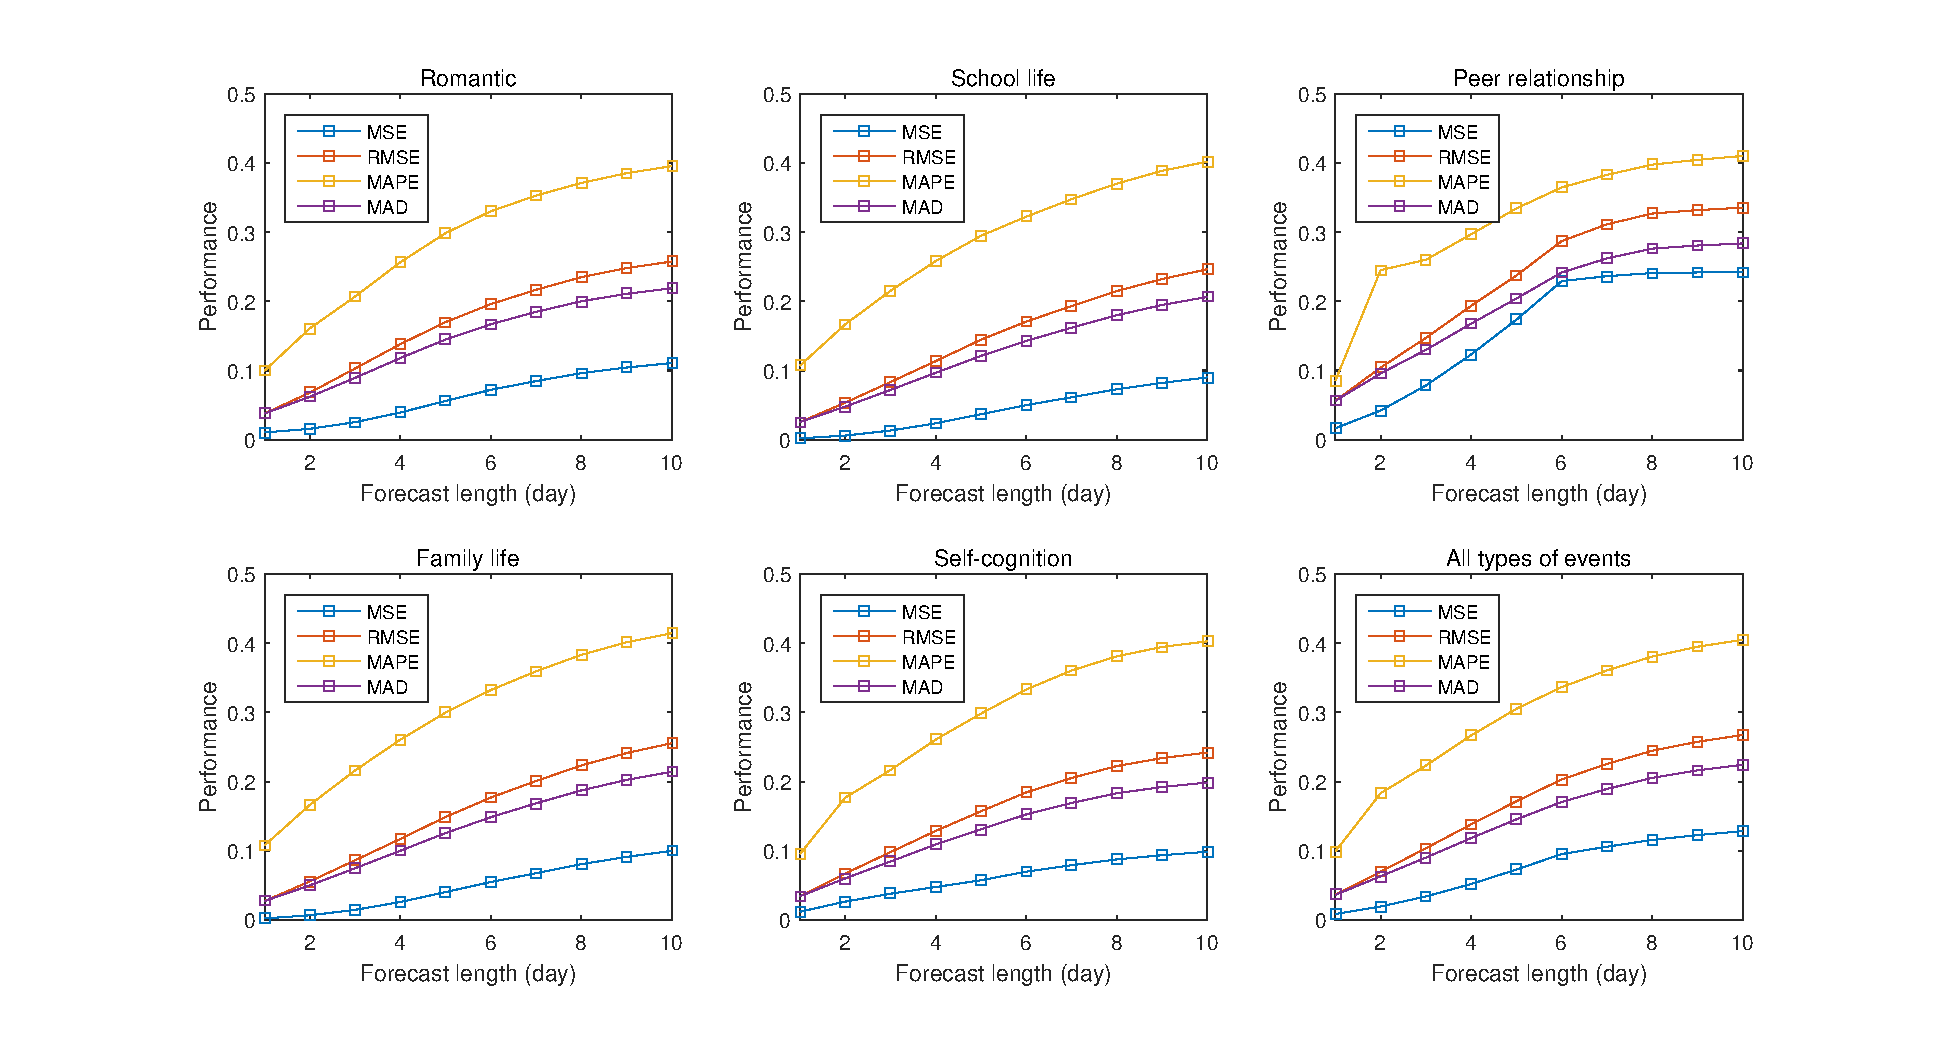
\includegraphics[width=\linewidth]{figs/predictWindow2.eps}
\label{fig:length}
\end{figure*}

\paragraph{Stress prediction performance under different observation window lengths}
We further explored combining stress-buffering effects into future stress prediction under different lengths of observation windows, ranging from 1 to 10 days, as shown in Figure \ref{fig:length}.
With increasing window length, the prediction errors showed an increasing trend across all the metrics.
The reason might be that a longer prediction window resulted in more previously predicted results and errors accumulating with more predicted values are taken into the next step of prediction.
Among the five dimensions of stressor events, the prediction for school-life stress achieved the best performance.
One reason might be that more positive events and stressors about school-life events were detected from adolescents' microblogs, providing sufficient data in the prediction process.
On the other hand, stress coming from school life was the most common source of stress in the student group 
with relatively stable periodicity,
which was more suitable for the current prediction model.


\begin{figure}
\centering
\caption{Stress prediction performance under the L\&S\&P stress-buffering pattern of positive events.}
\includegraphics[width=\linewidth]{figs/thresh.eps}
\label{fig:thresh}
\end{figure}

\paragraph{Parameter settings}
$\beta$ was adjusted when the impact of positive events was integrated into stress prediction.
For each of the four groups of stress-buffering patterns,
We adjust $\beta$ to the effect of $\beta \times L$.
%Editor: Please note that some text appears to be missing here. Please add any missing information:
{We calculated the corresponding prediction result for each adolescent as follows:}
and showed the result of the entire testing group in the average performance.
Figure \ref{fig:thresh} shows the changing trend under the L\&S\&P pattern.
The prediction errors decreased first and then increased,
and the best performance was achieved when $\beta$ was approximately0.52,
with an MSE of 0.0649, and RMSE of 0.2548, a MAPE of 0.2638 and a MAD of 0.0858 as the average performance of the entire experimental dataset.
Multiple methods for integrating the stress-buffering impact of positive events into stress prediction could be adopted in the future.
In this paper, we adopted a simple method to verify the effectiveness of our model in quantifying the impact of positive events.
The setting of $\beta$ could be changed according to different individuals and datasets.


\section{Discussion}
\label{sec:conclude}
The main contribution of the present study lies in the following three aspects.
First, we validated and expanded the theoretical results of previous studies.
The characteristics of stress buffering were not only manifested in self-reported subjective feelings but also at the behavioral level in social networks.
We examined the potential relationship between the occurrence of positive events and posting behaviors, microblog contents and stress-change modes on stressed adolescents,
and verified that positive events buffered monotonic changes in stress at both the early and late stages.
Second, this study implemented innovative methods.
Through building a complete technical framework,
we realized
1) the automatic extraction of positive events, as well as users' behaviors and content measures from microblogs
and 2) the quantification of relationships between the stress-buffering effects of positive events and microblogging measures.
Third, this article showed practical significance.
It realized the timely and continuous monitoring of the stress-buffering process
of adolescents based on public social network data sources,
which could be used to assess stress resistance in adolescents;
On the other hand, it could provide supplementary advice to schools and parents about when to schedule positive events to ease the stress of adolescents.

There were three groups of results in this work.
In study 1, the scheduled school events with exact time intervals and the microblogs posted by a group of 500 students were collected and statistically analyzed.
The results showed that when positive events were scheduled neighboring stressful events,
students exhibited less intense stress and shorter stressful time intervals based on their microblogs.
The study also found that most students talked less about the upcoming or just-finished exams when positive events occurred nearby, at a lower frequency and a lower ratio.
The results substantiated previous studies reporting the protective effect of positive events on adolescents~\citep{Cohen2010Positive,Shahar2002Positive} using laboratory methods.
Based on this conclusion, this article carried out more in-depth follow-up studies.

The second group of results was presented in study 2, which
examined the stress-buffering pattern of positive events through microblog content and behavioral measures.
A complete solution was provided for automatically detecting positive events based on microblog semantics, which were completely different from traditional questionnaire methods,
enabling timely, fraud-proof and continuous detection.
To eliminate possible errors in positive event detection and avoid false overlays,
We first used four positive scheduled events to examine significant stress-buffering effects.
The results showed that the event `holiday' exhibited the highest proportion of significant stress-buffering effects.
However, this conclusion was questionable because the frequencies of the above four events were different and might affect the experimental results.
Next, the stress-buffering effect of automatically extracted positive events was tested based on three groups of stress-buffering measures.
The most intensive stress-buffering effects were shown in the `school life' and `peer relationships' dimensions.
\emph{Posting behaviors} exhibited the most significant correlations among the three groups of measures.
This finding resonated with the study \cite{BLACHNIO2016664,Disclosure}, suggesting that users who tended to share important news on Facebook had a higher level of stress.

This article proposed a novel perspective to better understand the stress-buffering process.
Since more complex situations were simplified in the present exploration, 
the goals were still salient for stress-buffering studies from social networks.

\section{Limitations and future work}

This study has a number of limitations.
First, it used a microblog dataset collected from social networks of high school students,
and chose the scheduled school events as the ground truth in the pilot study.
This method could be seen as relative fuzzy verification,
because individual events (i.e., `lost love', or `received a birthday present') might also have additional impact.
Therefore, the data observations in the pilot study were not 100\% rigorous and need further verification.
An improvement might be implemented by inviting participants to complete related scales (e.g., positive and stressor scales) to label part of the dataset and achieve a balance between data volume and accuracy.

Second, this study treated positive events as independent and studied the effect of each event separately, which ignores the additive and collective effects of multiple positive events that might happen at the same time.
Thus, our future research might investigate the overlap effects of multiple positive events,
as well as the frequent coappearance patterns of different types of positive events to provide more accurate stress-buffering guidance for individual adolescents.

Based on our current research implications, more factors could help analyze stress-buffering patterns among adolescents more comprehensively in future research.
One factor is how personality ~\citep{personality1,personality2} impacts the stress-buffing effect of positive events, 
which could be captured from the social media contents.
Another key factor is the role social support~\citep{socialSupport1, socialSupport2} in social networks plays.
This factor leaves clues in the messages under each post,
and the behaviors (i.e., retweets and the number of likes) of friends.
For example, ~\citep{socialSupport1} showed that the number of Facebook friends was associated with stronger perceptions of social support,
which in turn correlated with reduced stress and greater sense of well-being.
The corresponding experimental design and the online/offline complementary verification will be challenges in future work.


\section{References}
%\bibliographystyle{model4-names}
%\bibliography{reference-new}
\end{document}
